\documentclass[a4paper, 12pt]{article}
\usepackage{listings} 
\usepackage{xcolor} 
\usepackage{mdframed}
\usepackage{graphicx}
\usepackage{pgfplots} % Making graphs
\usepackage{float} % Strict placement of tables and images
\usepackage{mathtools}
\usepackage[margin=1.00in]{geometry} % Margin setting
\usepackage{breqn} % Automatically breaking equation lines up
\usepackage[version=4]{mhchem}
\DeclarePairedDelimiter\ceil{\lceil}{\rceil}
\DeclarePairedDelimiter\floor{\lfloor}{\rfloor}

% Row operation matrix setup
\usepackage{amsmath,mathtools}
\newenvironment{sysmatrix}[1]
 {\left(\begin{array}{@{}#1@{}}}
 {\end{array}\right)}
\newcommand{\ro}[1]{%
  \xrightarrow{\mathmakebox[\rowidth]{#1}}%
}
\newlength{\rowidth}% row operation width
\AtBeginDocument{\setlength{\rowidth}{3em}}

\definecolor{code-gray}{gray}{0.93} % Nice background color for code boxes
\newcommand*\chem[1]{\ensuremath{\mathrm{#1}}} % Easy input of Chemical equations
\begin{document}
\title{Math 428 - Case Study\\\large Concentration of Brine in a 5-Tank System}
\author{Santiago Gutierrez, Collin Heist, Koffi Koffi, Kyle Luchte}
\date{\today}
\maketitle
\pagenumbering{roman}
\tableofcontents
\newpage
\pagenumbering{arabic}

\section{Case Description}
Brine is a general term used to refer to any salt (\chem{NaCl}) and water (\chem{H_2O}) solution. This can be represented by the chemical equation:
\begin{center}
\ce{NaCl(s) + H2O(l) = NaCl(aq)}
\end{center}

For this case study, we will study the system of interconnected tanks shown below in Figure \ref{fig:tanks}.

\begin{figure}[H]
\centering
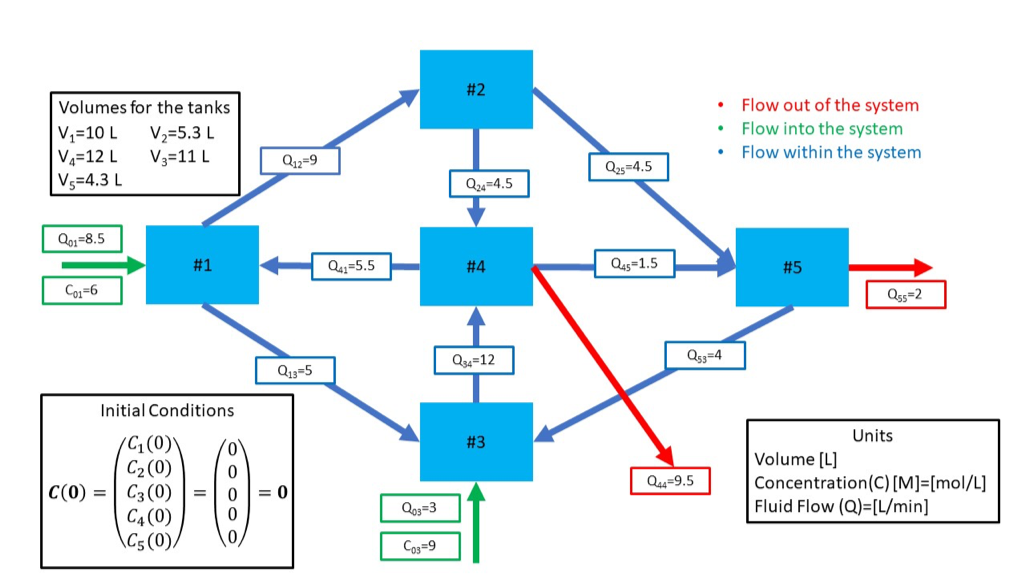
\includegraphics[width=.9\textwidth]{tankSystem.png}
\caption{Tank Diagram}
\label{fig:tanks}
\end{figure}

Initially, the fluid flow in the system is comprised entirely of water. However, at the push of a button a timer begins and a solution of brine flows into the system. Figure \ref{fig:tanks} has two points of entry for this brine solution, tank \#1 and \#3. The solution flows in at the specified rates and concentrations. Another assumption of this model is that the tanks are instantly homogeneous (i.e. the concentration of the brine in any given tank at one point in time is equal throughout the tank's entire volume). There are no leaks, clots, or effects of pressure or temperature on the system.

In this system, the provided flow rates are constant in time (and thus the volumes are constant as well). The result of these assumptions is that the concentration in each tank is the only parameter that changes as a function of time.

The reason to solve a system such as this could easily be found by extrapolating outwards. If you were a governmental organization hoping to monitor the flow of a toxin through a water supply system, this type of situation is perfectly applicable. Or, perhaps a chemical business would like to know how long it will take some tanks to reach a desired concentration needed for a certain process, this type of case study would also be insightful there as well.

\section{Definitions}
There are many relevant definitions that are used throughout this case study
\begin{itemize}
\item $Q_{ij}$ is the flow from tank \textbf{i} to \textbf{j}. When $i=0$, this indicates flow \textit{into} the system, and when $i=j$, this indicates flow \textit{out} of the system.
\item $C_i(t)$ is the concentration in tank \textbf{i}. This is equivalent to $\frac{x_i(t)}{V_i}$
\item Accumulation is defined as
$$V_i\frac{dc_i}{dt}=\sum_{k=0}^{5} Q_{ki}C_k-\sum_{l=0}^{5} Q_{il}C_i$$
\item \textbf{i} is the tank index. This can be a value between 1 and 5.
\end{itemize}

\section{Objectives and Involved Numerical Methods}
Below are the four main objectives of this case study:
\begin{enumerate}
\item Find the value the concentrations approach as time progresses. This is represented as follows:
$$\lim_{t\to\infty}C_i(t)$$
This is the steady-state solution obtained through \textbf{Gaussian Elimination}.
\item Find the concentration of salt inside each tank. This is the numerical solution for $C_i(t)=\frac{x_i(t)}{V_i}$ obtained through the \textbf{$4^{th}$ order Runge-Kutta method}.
\item Find the analytical solution for the system of equations by applying the Eigenvalue Method and the Method of Undetermined Coefficients to the following system of differential equations:
$$C'(t)=R\cdot C(t)+b_2$$
\item Verify the validity of the numerical solution by comparing it to the analytical and steady-state solutions.
\end{enumerate}


\section{Relevant Equations}
As $t \rightarrow \infty$, each $C_i$ approaches the steady state solution.
\begin{align}
	\begin{bmatrix}
		V_1\cdot C_1'(t) \\
		V_2\cdot C_2'(t) \\
		V_3\cdot C_3'(t) \\
		V_4\cdot C_4'(t) \\
		V_5\cdot C_5'(t) \\
	\end{bmatrix} = Q\cdot C(t)+b_1 =
	\begin{bmatrix}
		-14 & 0 & 0 & 5.5 & 0\\
		9 & -9 & 0 & 0 & 0\\
		5 & 0 & -12 & 0 & 4\\
		0 & 4.5 & 12 & -16.5 & 0 \\
		0 & 4.5 & 0 & 1.5 & -6
	\end{bmatrix}
	\begin{bmatrix}
		C_1(t)\\C_2(t)\\C_3(t)\\C_4(t)\\C_5(t)
	\end{bmatrix} +
	\begin{bmatrix}
		51\\0\\27\\0\\0
	\end{bmatrix}
\end{align}

Below is the linear system used to solve the steady state solution. $C_{if}$ is the final concentration in each tank.
\begin{align}
	Q\cdot C_{final}=-b_1=
	\begin{bmatrix}
		-14 & 0 & 0 & 5.5 & 0\\
		9 & -9 & 0 & 0 & 0\\
		5 & 0 & -12 & 0 & 4\\
		0 & 4.5 & 12 & -16.5 & 0 \\
		0 & 4.5 & 0 & 1.5 & -6
	\end{bmatrix}
	\begin{bmatrix}
		C_{1f}\\C_{2f}\\C_{3f}\\C_{4f}\\C_{5f}
	\end{bmatrix} =
	\begin{bmatrix}
		-51\\0\\-27\\0\\0
	\end{bmatrix}
\end{align}

\begin{align}
	\begin{bmatrix}
		C'_1(t)\\C'_2(t)\\C'_3(t)\\C'_4(t)\\C'_5(t)
	\end{bmatrix} = R\cdot C(t)+ b_2 = 
	\begin{bmatrix}
		\frac{-14}{V_1} & 0 & 0 & \frac{5.5}{V_1} & 0\\
		\frac{9}{V_2} & \frac{-9}{V_2} & 0 & 0 & 0\\
		\frac{5}{V_3} & 0 & \frac{-12}{V_3} & 0 & \frac{4}{V_3}\\
		0 & \frac{4.5}{V_4} & \frac{12}{V_4} & \frac{-16.5}{V_4} & 0 \\
		0 & \frac{4.5}{V_5} & 0 & \frac{1.5}{V_5} & \frac{-6}{V_5}
	\end{bmatrix}
	\begin{bmatrix}
		C_1(t)\\C_2(t)\\C_3(t)\\C_4(t)\\C_5(t)
	\end{bmatrix} +
	\begin{bmatrix}
		\frac{51}{V_1}\\0\\\frac{27}{V_3}\\0\\0
	\end{bmatrix}
\end{align}

$\lambda_i$ is the eigenvalue for each tank.

\begin{align}
	\begin{vmatrix}
		\frac{-14}{V_1}-\lambda_1 & 0 & 0 & \frac{5.5}{V_1} & 0\\
		\frac{9}{V_2} & \frac{-9}{V_2}-\lambda_2 & 0 & 0 & 0\\
		\frac{5}{V_3} & 0 & \frac{-12}{V_3}-\lambda_3 & 0 & \frac{4}{V_3}\\
		0 & \frac{4.5}{V_4} & \frac{12}{V_4} & \frac{-16.5}{V_4}-\lambda_4 & 0 \\
		0 & \frac{4.5}{V_5} & 0 & \frac{1.5}{V_5} & \frac{-6}{V_5}-\lambda_5
	\end{vmatrix} = 0
\end{align}
\section{Analysis}
\subsection{Objective 1}
As time goes by and the conditions of the system remains unchanged, the whole system approaches a balanced state called its steady-state. Once the steady-state is reached, the concentrations of salt inside each of the tanks remain constant (meaning the derivatives of the concentrations become zero). Thus, \textbf{Equation 2} will be used to find the steady-state solution. Using the attached \textbf{Code A} $C_{final}$ is found as:

\begin{align}
	C_{final}=	
	\begin{bmatrix}
		C_{1f}\\C_{2f}\\C_{3f}\\C_{4f}\\C_{5f}
	\end{bmatrix}=
	\begin{bmatrix}
		6.33389544688027\\6.33389544688027\\7.04342327150084\\6.84991568296796\\6.46290050590219
	\end{bmatrix}
\end{align}

These results represent the final concentrations of each tank as time approaches infinity. However, because of the flow rates for this problem, the system converges relatively quickly and can be approximated numerically; as shown in \textbf{Objective 2}.

\subsection{Objective 2}
In order to find the concentration of salt inside each tank, we implemented the $4^{th}$ order Runge-Kutta method for a system of equations. Specifically \textbf{Equation 3} allows the concentration at each point in time to be identified. Using \textbf{Code B}, the in and outflows of the tank system was modeled using five separate functions, and then the RK4 method was used to compute the concentration in each tank at each point in time. Because one tank does not reach equilibrium, followed by another, and the rest (one at a time), and instead each mixing of the tank occurs to \textit{all} the tanks simultaneously, the RK method is used on the five equations simultaneously. This is equivalent to one unit of time passing for all the tanks together.

The results of this are shown in \textbf{Code B}, but Figure \ref{fig:numerical-sol} is the graphical representation of the concentrations in each tank over time:

\begin{figure}[H]
\centering
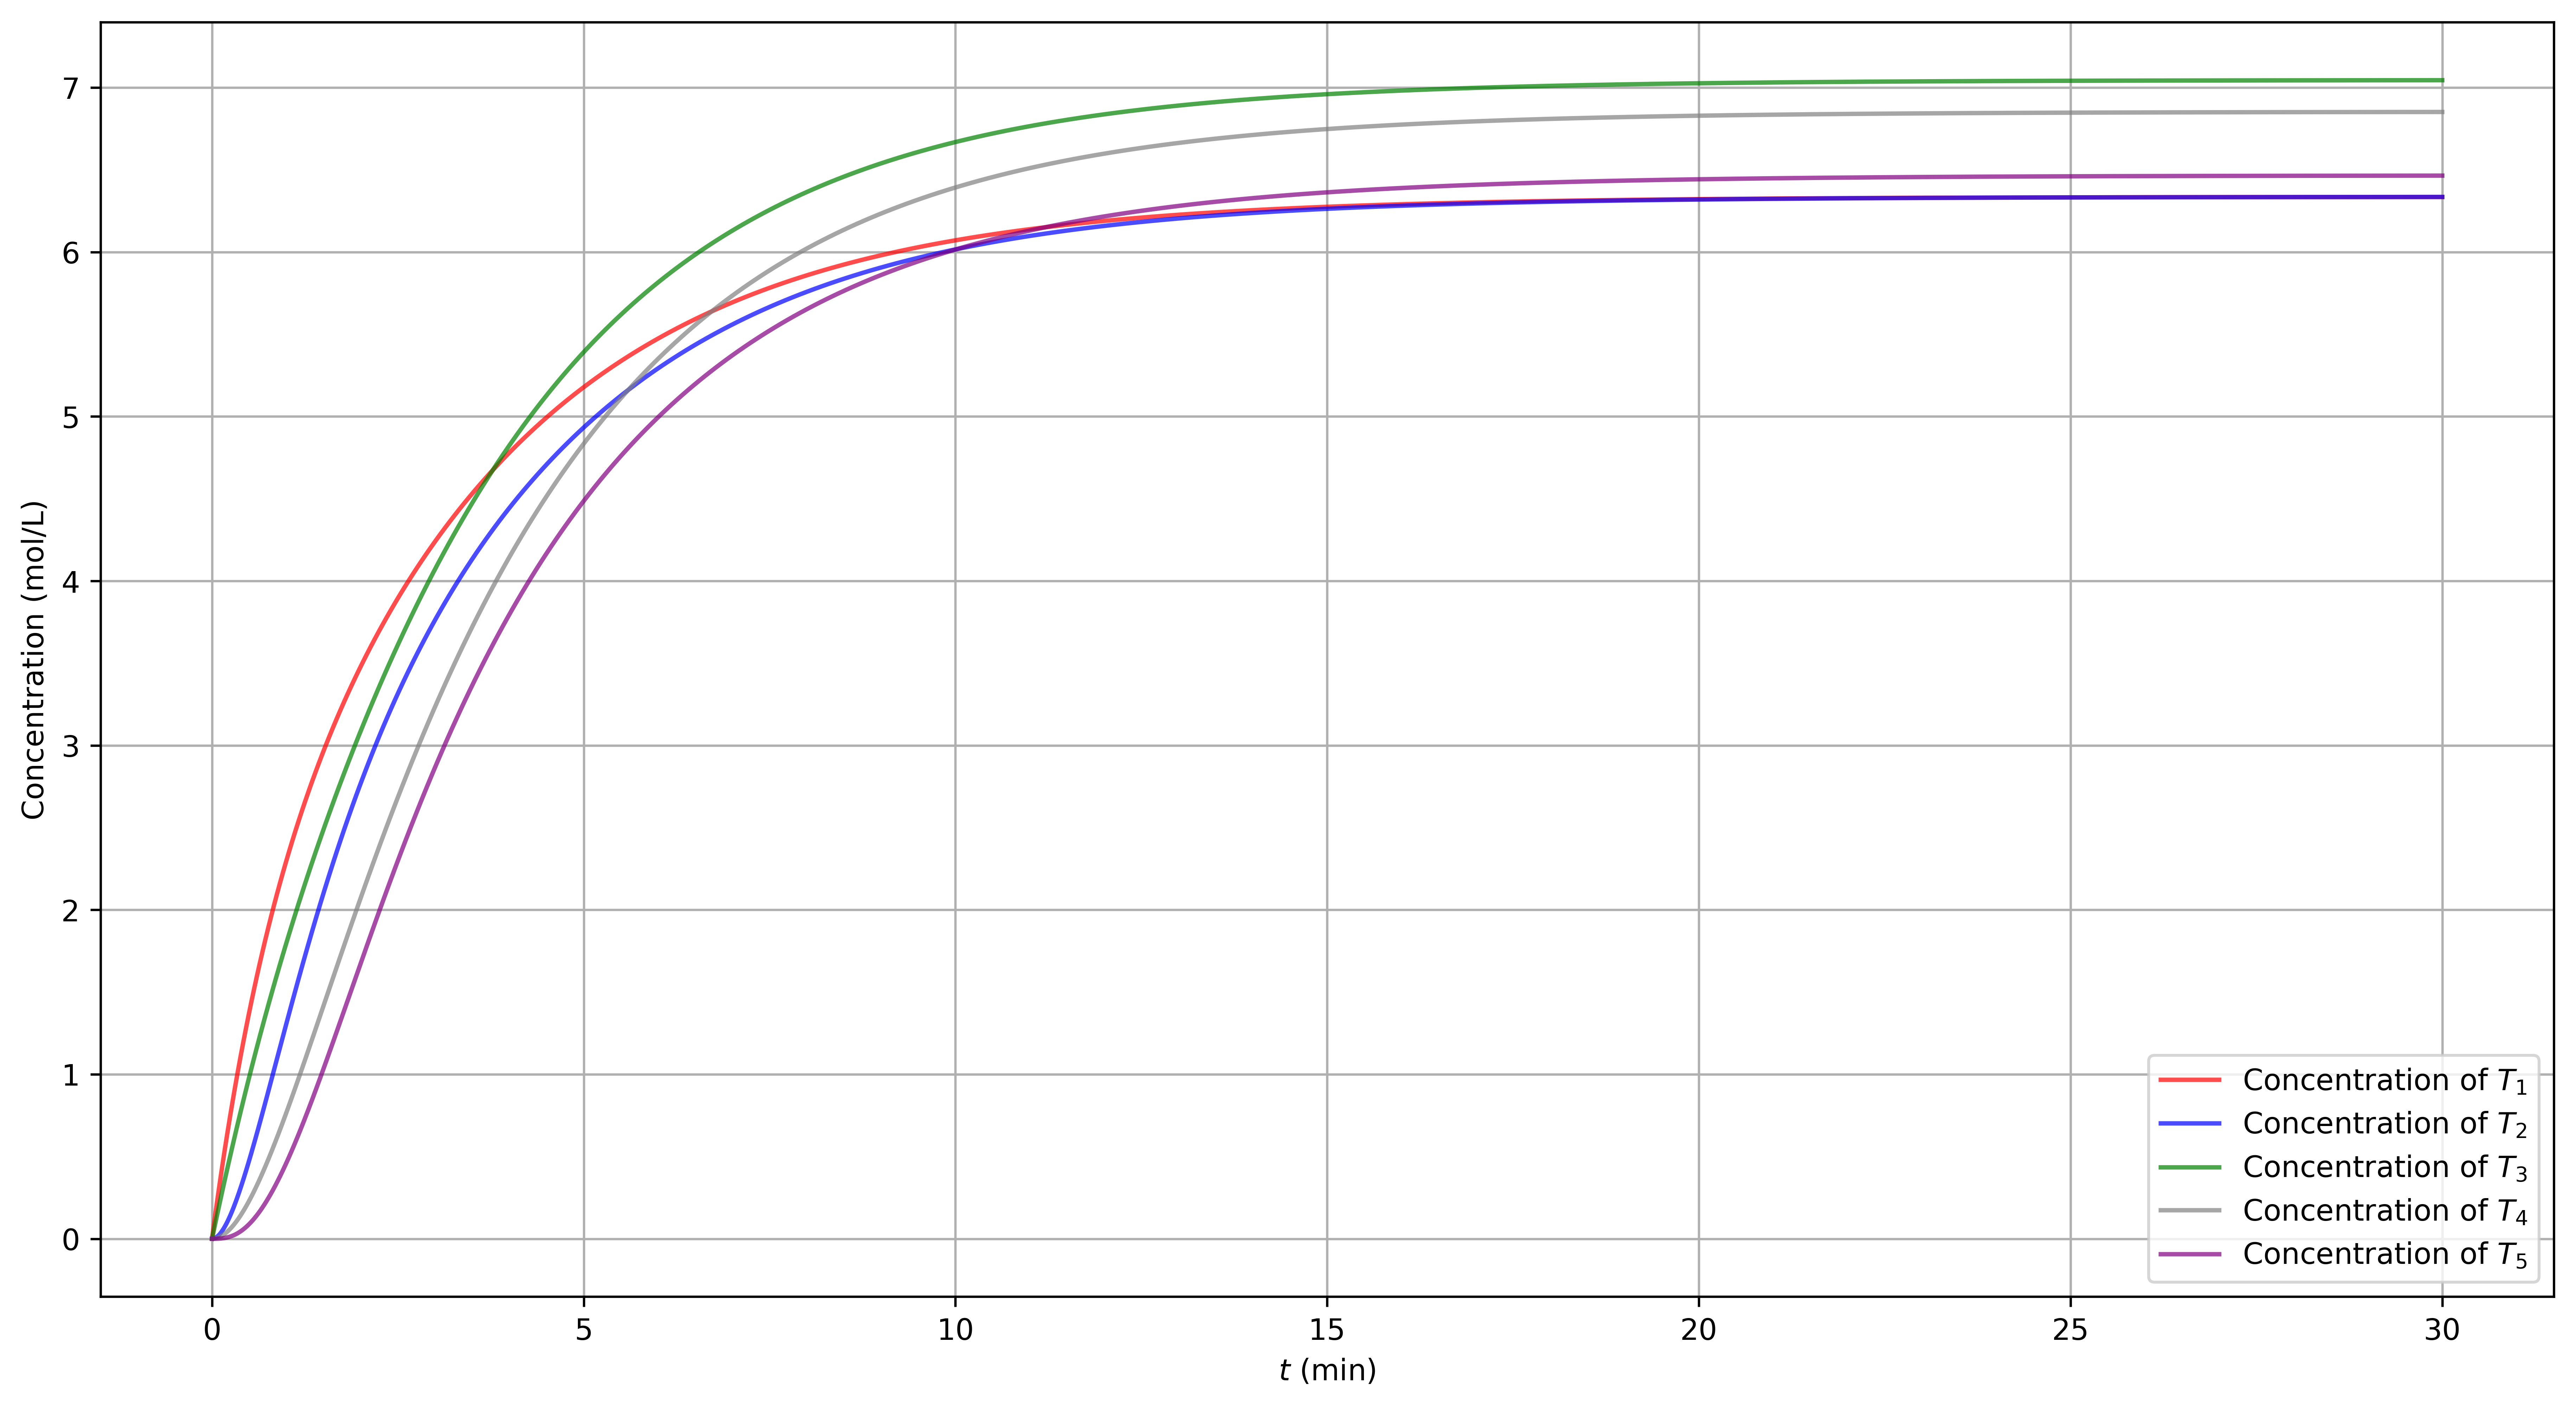
\includegraphics[width=.9\textwidth]{NumericalSol.png}
\caption{Concentration in each tank over time (numerically found with RK4)}
\label{fig:numerical-sol}
\end{figure}

Given the physical conditions of the problem, the found numerical results make sense. It is logically consistent with the problem statement that after a set amount of time the concentration inside each tank reaches an equilibrium (as their volumes are constant, as is the inflow of brine into the system). 

\subsection{Objective 3}
\textbf{Equation 3} is a nonhomogenous linear system of ordinary differential equations with constant coefficients; this implies that the solution, $C(t)$, has two parts called the complementary and particular solutions. These exist such that
\begin{equation}
C(t)=C_c(t)+c_p
\end{equation}
The complementary solution can be derived by applying the Eigenvalue Method. This method requires us to find the Eigenvalues of \textbf{R} seen in \textbf{Equation 4} and the corresponding Eigenvectors. This was accomplished using Matlab, as shown in \textbf{Code C}. The results are as follows:

\begin{align}
	Eigenvalues = 
	\begin{bmatrix}
		\lambda_1\\\lambda_2\\\lambda_3\\\lambda_4\\\lambda_5\\
	\end{bmatrix}=
	\begin{bmatrix}
		-0.34161338483812 + 0i \\-2.01213779895561+0.679814462137368i \\
		-2.01213779895561-0.679814462137368i \\ -1.29674107645811 + 0.62513266343316i \\
		-1.29674107645811 - 0.62513266343316i \\
	\end{bmatrix}
\end{align}

Eigenvectors:
\begin{align}
	V_1 = 
	\begin{bmatrix}
		-0.287319340730301+0i\\-0.3596762484668+0i\\-0.436480762081284+0i\\-0.552899899101974+0i\\
		-0.540247016314873+0i
	\end{bmatrix}
\end{align}
\begin{align}
	V_2=
	\begin{bmatrix}
		0.0400359558124153+0.25065825298207i\\0.4808412447767707-0.252065825298207i\\
		0.203658175482949+0.0259158205576298i\\-0.356119118760743-0.231058177678548i\\
		-0.6144376403809+0.0i\\
	\end{bmatrix}
\end{align}
\begin{align}
	V_3 = 
	\begin{bmatrix}
		0.0400359558124153-0.252065825298028i\\0.480841244776707+0.252065825298028i\\
		0.203658175482949-0.02515805576298i\\-0.356119118760743+0.231058177678548i\\
		-0.6144376403809+0.0i
	\end{bmatrix}
\end{align}
\begin{align}
	V_4=
	\begin{bmatrix}
		-0.14357345203895+0.165140649023423i\\0.140332766676723+0.480105383717494i\\
		0.0132079479842168-0.324571574695876i\\-0.214654634610346-0.132182144622021i\\
		0.729966362220564+0i
	\end{bmatrix}
\end{align}
\begin{align}
	V_5=
	\begin{bmatrix}
		-0.143573405203895-0.165140649023423i\\0.140332766676723-0.480105383717494i\\
		0.0132079479842168+0.3245715774695876i\\-0.214654634610346+0.132182144622021i\\
		0.729966362220564+0i
	\end{bmatrix}
\end{align}

Notice that $\lambda_1$ and its corresponding eigenvector are strictly real while $(\lambda_2,\lambda_3)$ and $(\lambda_4,\lambda_5)$ are complex conjugates. This implies the complementary solution, $C_c(t)$ has three components:
\begin{equation}
C_1(t)=V_1e^{\lambda_1t}
\end{equation}
\begin{equation}
C_2(t)=e^{Re(\lambda_2)t}\cdot(Re(V_3)cos(Im(\lambda_2)t)+Im(V_3)sin(Im(\lambda_2)t))
\end{equation}
\begin{equation}
C_3(t)=e^{Re(\lambda_2)t}\cdot(Im(V_3)cos(Im(\lambda_2)t)-Re(V_3)sin(Im(\lambda_2)t))
\end{equation}
\begin{equation}
C_4(t)=e^{Re(\lambda_4)t}\cdot(Re(V_5)cos(Im(\lambda_4)t)+Im(V_5)sin(Im(\lambda_4)t))
\end{equation}
\begin{equation}
C_5(t)=e^{Re(\lambda_4)t}\cdot(Re(V_5)cos(Im(\lambda_4)t)-Im(V_5)sin(Im(\lambda_4)t))
\end{equation}
Where the complementary solution is the sum of these parts, shown as:
\begin{equation}
C_c(t)=C_1(t)+C_2(t)+C_3(t)+C_4(t)+C_5(t)
\end{equation}

On the other hand, the \textit{particular} solution can be found using the Method of Variation of Parameters. Since $b_2$ is a constant coefficient vector, $c_p=(a_1, a_2, a_3, a_4, a_5)^T$. Substituting $c_p$ into \textbf{Equation 3} yields:

\begin{equation}
\frac{d}{dt}c_p=R\cdot c_p+b_2=0\rightarrow R\cdot c_p=-b_2\rightarrow (R|-b_2)
\end{equation}

Notice that $(Q|-b_2)$ ~ $(R|-b_2)$, as can be shown below:

\begin{alignat*}{2}
	\begin{sysmatrix}{rrrrr|r}
		-14 & 0 & 0 & 5.5 & 0 & -51 \\
		9 & -9 & 0 & 0 & 0 & 0 \\
		5 & 0 & -12 & 0 & 4 & -27 \\
		0 & 4.5 & 12 & -16.5 & 0 & 0 \\
		0 & 4.5 & 0 & 1.5 & -6 & 0 \\
	\end{sysmatrix}
	&\!\begin{aligned}
	&\ro{R_1/V_1}\\
	&\ro{R_2/V_2}\\
	&\ro{R_3/V_3}\\
	&\ro{R_4/V_4}\\
	&\ro{R_5/V_5}\\
	\end{aligned}
	\begin{sysmatrix}{rrrrr|r}
		\frac{-14}{V_1} & 0 & 0 & \frac{5.5}{V_1} & 0 & \frac{51}{V_1}\\
		\frac{9}{V_2} & \frac{-9}{V_2} & 0 & 0 & 0 & 0\\
		\frac{5}{V_3} & 0 & \frac{-12}{V_3} & 0 & \frac{4}{V_3} & \frac{27}{V_3}\\
		0 & \frac{4.5}{V_4} & \frac{12}{V_4} & \frac{-16.5}{V_4} & 0 & 0 \\
		0 & \frac{4.5}{V_5} & 0 & \frac{1.5}{V_5} & \frac{-6}{V_5} & 0
	\end{sysmatrix}
\end{alignat*}

Because the two augmented matrices are row equivalent, they represent the same system and share a solution set. This implies that $c_p$ is the steady state solution. Hence, using Gaussian Elimination with partial pivoting, shown in \textbf{Code A}, the steady state solution is found to be:

\begin{align}
	c_p=	
	\begin{bmatrix}
		C_{1f}\\C_{2f}\\C_{3f}\\C_{4f}\\C_{5f}
	\end{bmatrix}=
	\begin{bmatrix}
		6.33389544688027\\6.33389544688027\\7.04342327150084\\6.84991568296796\\6.46290050590219
	\end{bmatrix}
\end{align}

Thus, a solution for \textbf{Equation 3} can be found by applying the Principle of Linear Superposition, arriving at:

\begin{equation}
C(t)=C_c(t)+c_p=w_1C_1(t)+w_2C_2(t)+w_3C_3(t)+w_4C_4(t)+w_5C_5(t)+c_p
\end{equation}

Applying the initial conditions, and defining \textbf{w} as:

\begin{equation}
C(0)=C_c(0)+c_p=0\rightarrow C_c(0)=-c_p\rightarrow (C_1(0) C_2(0) C_3(0) C_4(0) C_5(0) | -c_p)
\end{equation}
\begin{align}
	w=
	\begin{bmatrix}
		w_1\\w_2\\w_3\\w_4\\w_5\\
	\end{bmatrix}=
	\begin{bmatrix}
		16.0969656124024\\-2.58567417344085\\4.62001300762691\\0.883193573519296\\1.90174535349253
	\end{bmatrix}
\end{align}

In order to arrive at the concentration in each tank one only needs to break up the concentration matrices into their row-by-row equivalents (so row 1 is tank 1, etc.). This allows for a generic analytic solution to be found as:

\begin{dmath}
c_i(t)=p_{i1}e^{\lambda_1t}+e^{Re(\lambda_2)t}(p_{i2}cos(Im(\lambda_2)t)+p_{i3}sin(Im(\lambda_2)t))+e^{Re(\lambda_4)t}(p_{i4}cos(Im(\lambda_4)t)+p_{i5}sin(Im(\lambda_4)t))
\end{dmath}

Wherein $p_{ij}$ values are given below, and calculated from \textbf{Code C}.

\begin{align*}
	p_1 = 
	\begin{bmatrix}
		-4.624969\\ -1.268067\\ 0.466793\\ -0.440859\\ 0.127189
	\end{bmatrix},
	p_2=
	\begin{bmatrix}
		-5.789696\\ 0.244898\\-3.054389\\ -0.789097\\ -0.690903
	\end{bmatrix},
	p_3 = 
	\begin{bmatrix}
		-7.026016\\ -0.646325\\ -0.873894\\ 0.626964\\ 0.261541
	\end{bmatrix}
\end{align*}
\begin{align*}
	p_4=
	\begin{bmatrix}
		-8.900011\\ 1.988299\\ 1.047834\\ 0.061795\\ 0.52500
	\end{bmatrix},
	p_5=
	\begin{bmatrix}
		-8.696338\\ 1.588736\\ 2.838709\\ 0.644706\\ -1.388210
	\end{bmatrix}
\end{align*}

\subsection{Objective 4}
Attached, in \textbf{Code D}, is the Python code used to compare the numerical solution to both the steady state and analytical solutions. The values listed in the previous section were used are comparison. However, the following two plots (Figures \ref{fig:num-vs-steady} and \ref{fig:num-vs-anal}) are the most important findings from this analysis:

\begin{figure}[H]
\centering
\includegraphics[width=.9\textwidth]{NumericalVsSteadyState.png}
\caption{Comparison of the numerical RK4 approximation to the steady state solution}
\label{fig:num-vs-steady}
\end{figure}

\begin{figure}[H]
\centering
\includegraphics[width=.9\textwidth]{NumericalVsAnalytical.png}
\caption{Comparison of the numerical RK4 approximation to the analytical solution}
\label{fig:num-vs-anal}
\end{figure}

A clear deviation of the numerical solution from the analytical solution can be seen in Figure \ref{fig:num-vs-anal}, and this is likely a result of the imprecision of the Runge-Kutta method. Despite using a small step size, there is still significant roundoff and truncation error present in all steps of the numerical method. However, this inaccuracy goes away as the system converges on its steady state solution, and the approximation becomes much more accurate.

\section{Results and Conclusion}
The results of this case study show that in the given five-tank Brine system, the tanks all converge to (nearly) their steady state systems after \textit{around} 20 minutes. This is particularly evident in Figure \ref{fig:numerical-sol}. As was demonstrated three ways (numerically, analytically, and with Gaussian Elimination), the tanks converge to the approximate values of 6.334, 6.334, 7.043, 6.850, and 6.463 moles of NaCl per Liters (for tanks 1 through 5 respectively). The exact values of the concentration at each point in time, as found through the numerical solution, clearly exhibit error when compared to the analytical solution. And, as discussed before, this is a result of the implicit uncertainty of representing floating point numbers on a computer, and the imprecision of using an approximating method (Runge-Kutta in this instance) to numerically solve systems of equations.

Despite these errors, we are confident that the above-listed methods are still very mathematically sound and appropriate ways to solve a problem such as this.

\end{document}